\documentclass[11pt]{article}

% Change "review" to "final" to generate the final (sometimes called camera-ready) version.
\usepackage[final]{acl}

\usepackage{times}
\usepackage{latexsym}
\usepackage[T1]{fontenc}
\usepackage[utf8]{inputenc}
\usepackage{microtype}
\usepackage{inconsolata}
\usepackage{graphicx}
\usepackage{booktabs}
\usepackage{amsmath}
\usepackage{multirow}
\usepackage{array}
\usepackage{xcolor}

\definecolor{goodgreen}{HTML}{2E7D32}
\newcommand\todo[1]{\textcolor{red}{#1}}

\title{Extracting Social and Clinical Impacts of Substance Use\\
from Reddit with Structured Pipelines and Ensemble Search}

\author{Ismail Elyamany, \ Chongtian Huang, \ Yitong Xia, \ Ruijie Zhu\\
Nanyang Technological University \\
\texttt{\{ismailma001, chongtia002, yitong010, ruijie008\}@e.ntu.edu.sg}
% \\ \todo{Everyone plz check your own email address}
}

\begin{document}
\maketitle

\begin{abstract}
We present our solution to the SMM4H--HeaRD 2026 Task~7,
which requires us to extract \emph{Clinical} and \emph{Social} impacts of
substance use from Reddit posts as a token-level BIO tagging problem. 
% The benchmark is difficult for two reasons: the label prior flips between train
% and test (train is $\approx$75\% Clinical, test is $\approx$70\% Social),
% and many entities are implicit colloquialisms without medical vocabulary.
We compare five model families---BiLSTM--CRF, GLiNER, SocBERT,
StressRoBERTa, and DeBERTa-v3-large---under a consistent learning-rate
sweep, and organize our contributions into seven buckets: classical loss and
prompt ablations, advanced regularization, a \emph{preprocessing axis}
treating raw and cleaned Reddit text as two experimental regimes,
four structured-prediction pipelines, domain-adapted backbones, weight-space
model soup, and an exhaustive prediction-space ensemble search. 
% Our best single model is definition prompting at relaxed F1 $= 0.613$. 
The final model is a four-model majority-vote ensemble with a relaxed F1 of $ 0.635$, beating the best published baseline on the same dev split by $+0.025$. 
% The main lesson is that training-objective diversity, combined
% with hard majority voting, is a stronger lever than polishing any single
% model.
\end{abstract}

\section{Introduction}

Public-health surveillance on social media has become an important source of population-level signals for substance-use disorders. The SMM4H--HeaRD 2026 task~7 asks participants to extract, from opioid-subreddit posts, two kinds of consequences that users describe in natural language: \emph{ClinicalImpacts} (physiological and psychological effects such as overdose or withdrawal) and \emph{SocialImpacts} (occupational, legal, and relational consequences such as losing a job or getting arrested). The task is formulated as token-level NER with five BIO tags: \texttt{O}, \texttt{B/I-ClinicalImpacts}, \texttt{B/I-SocialImpacts}.

What makes this benchmark unusually difficult is a striking mismatch
between the training and test distributions. The training split is
dominated by Clinical entities ($\approx$75\%) and the test split flips
to Social ($\approx$70\%). On top of that, many impacts are expressed
\emph{implicitly}---``those weeks were hell'' is a Clinical span without
a single clinical token---so lexical and ontology-based cues are weak. The
best published baseline on this split \citep{dey2025reddit}, a
DeBERTa-large \citep{he2023debertav3} token classifier, reaches relaxed F1
$= 0.610$.

We treat this as a systems problem and report a thorough comparison across
five model families under a uniform LR sweep and a paired \emph{raw vs preprocessed} protocol. Our contributions are:

\begin{enumerate}
\itemsep0em
\item A disciplined baseline study across BiLSTM--CRF, GLiNER
fine-tuned, SocBERT, StressRoBERTa, and DeBERTa-v3-large, showing that a
general-purpose encoder dominates Reddit- and mental-health-adapted
encoders on this task (\S\ref{sec:models}).
\item A \emph{preprocessing-as-axis} design in which every single model is
run in both a raw-text regime and a mojibake/URL/emoji-cleaned regime, so preprocessing is a first-class experimental variable rather than a
confound (\S\ref{sec:preproc}).
\item Seven contributions layered around a DeBERTa backbone:
(1) loss, prompt, and multi-task ablations (focal loss, definition
prompting, multi-task auxiliary head); (2) advanced regularisation
(recall-boost \texttt{O}-downweighting, R-Drop, Fast Gradient Method
(FGM) $+$ Stochastic Weight Averaging (SWA)); (3) preprocessing as a
first-class axis applied to all families (\S\ref{sec:preproc}); (4) four
structured prediction pipelines; (5) domain-adapted backbones (SocBERT,
StressRoBERTa); (6) weight-space model soup; and (7) an exhaustive
prediction-space ensemble search (\S\ref{sec:methods}).
\item An exhaustive ensemble search across both preprocessing regimes. A
four-model majority-vote ensemble reaches relaxed F1 $= \textbf{0.635}$ on
the dev set, exceeding the published baseline by $+0.025$ on the same
split (\S\ref{sec:ensemble}).
\end{enumerate}

The clearest single takeaway from the study is that \emph{training-objective diversity} is worth more than squeezing an additional point out of any
individual recipe. Five of the seven individual innovations sit at or
below the plain DeBERTa baseline when measured alone; they earn their
keep by producing decorrelated errors that hard voting combines.

\section{Related Work}
\label{sec:related}

\paragraph{Health-focused NER on social media.}
Extracting clinically relevant spans from social media text has been
studied for medication mentions, adverse drug events, and more recently
substance-use impacts \citep{sarker2019social,weissenbacher2022overview,
dey2025reddit}. The dominant approach is a transformer encoder with a
token-classification head, sometimes augmented with domain adaptation.
Reddit-Impacts~2.0 \citep{dey2025reddit} is unusual in separating \emph{clinical} and \emph{social} outcomes and in deliberately flipping the label prior between train and test.

\paragraph{Domain-adapted encoders.}
Reddit-specific pre-training \citep{guo2023socbert} and mental-health-domain pre-training \citep{stressroberta2022} typically help when the downstream task shares vocabulary and register with the pre-training corpus. In our setting, however, the task labels are not register-bound and generic
DeBERTa-v3 \citep{he2023debertav3} outperforms both domain-adapted encoders.

\paragraph{Span-based NER.}
GLiNER \citep{zaratiana2024gliner} frames NER as open-type span
scoring and is attractive for low-resource settings. We include both
zero-shot and fine-tuned variants, and a span-nested decoder that scores
nested candidates explicitly.

\paragraph{Regularisation and ensembling.}
Our advanced regularisation bucket is built from off-the-shelf
ingredients: focal loss \citep{lin2017focal}, R-Drop consistency
\citep{liang2021rdrop}, FGM adversarial training
\citep{miyato2017adversarial}, and SWA \citep{izmailov2018swa}.
Model soup \citep{wortsman2022modelsoup} and prediction-space ensembles
\citep{kuncheva2003measures} are well-established; our contribution is
the exhaustive cross-regime subset search.

\section{Task and Dataset}
\label{sec:data}

\paragraph{Reddit-Impacts 2.0.} The dataset contains $1{,}378$ posts from
opioid-related subreddits, pre-split into train, dev ($258$ posts), and
test. The training and dev splits are both Clinical-heavy, while the
test split flips to roughly 70\% Social. Figure~\ref{fig:eda} visualizes the split
composition, the span-length distribution, and the fraction of posts that
contain no entities at all (a non-trivial class, particularly on dev).

\begin{figure*}[t]
\centering
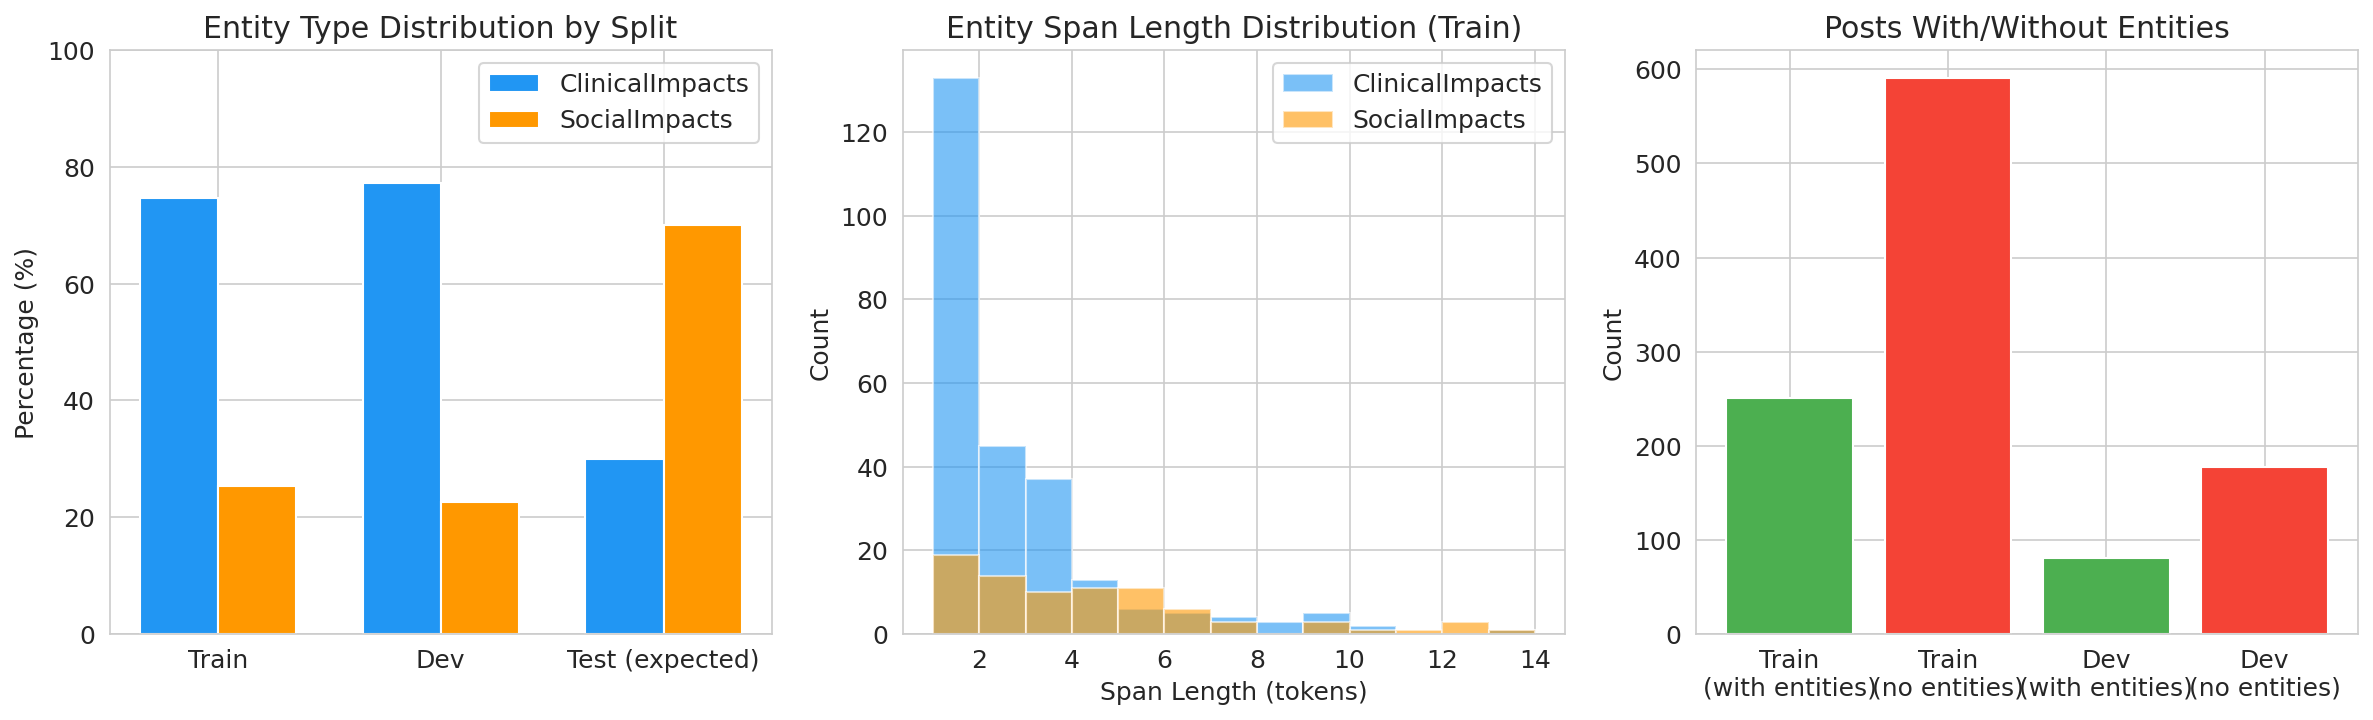
\includegraphics[width=\linewidth]{fig_eda.png}
\caption{Reddit-Impacts 2.0 exploratory statistics. \textbf{Left:}
Train/Dev are Clinical-heavy; Test flips to $\approx$70\% Social.
\textbf{Middle:} Social spans are longer and heavier-tailed than
Clinical. \textbf{Right:} the majority of dev posts contain no entities
at all, which makes a sentence-level presence head a useful auxiliary
signal.}
\label{fig:eda}
\end{figure*}

\paragraph{Evaluation.} We report both Relaxed and Strict F1 over entity
mentions. Relaxed F1 credits a prediction whose type is correct and whose
span overlaps the gold span by at least one token; Strict F1 additionally
requires exact span boundaries. Dev-set performance is the primary
selection criterion because test-set labels are not available; we discuss
the implications of this in \S\ref{sec:limit}.

\section{Preprocessing as an Axis}
\label{sec:preproc}

A common pitfall in social-media NER is to conflate preprocessing with
modeling: a single ``cleaned'' pipeline is used for every experiment and its effect is invisible. We treat preprocessing as a first-class
experimental axis. Every family is run twice:

\begin{itemize}
\itemsep0em
\item \textbf{Raw regime.} Original Reddit text goes straight to the tokenizer. Usernames, URLs, mojibake (broken Unicode from earlier
encoding/decoding trips), emoji, and stray punctuation are preserved.
This regime maximizes lexical fidelity but produces noisy token
boundaries.
\item \textbf{Preprocessed regime.} We repair mojibake, mask
\texttt{@user} mentions and URLs with placeholder tokens, strip emoji and
long punctuation runs, and restore masked positions as \texttt{O} tags at
inference time so that the BIO sequence length is preserved.
\end{itemize}

The effect of the regime is family-specific. BiLSTM--CRF and GLiNER both
gain markedly from preprocessing (relaxed F1 $+0.045$ and $+0.061$
respectively). The plain DeBERTa baseline is actually \emph{stronger} on
raw text ($0.595$ vs $0.545$), which is consistent with the hypothesis
that large pre-trained encoders are already robust to Reddit-style noise
and that aggressive cleaning removes genuine signal. Conversely,
definition prompting and R-Drop only become their best selves in the
preprocessed regime, because both rely on stable attention over a clean
context. This asymmetry is exactly why treating preprocessing as an
axis matters.

\section{Methods}
\label{sec:methods}

\subsection{Model families}
\label{sec:models}

\paragraph{BiLSTM--CRF (sanity check).} A frozen GloVe-300d embedding
layer feeds a two-layer BiLSTM ($2{\times}256$), a linear projection to
five tags, and a CRF with Viterbi decoding at inference time.

\paragraph{GLiNER.} We include two variants of GLiNER
\citep{zaratiana2024gliner}: (a) fine-tuned on Reddit-Impacts with a
$0.3$ span-score threshold; and (b) a span-nested variant that enumerates
nested candidate spans and applies overlap-aware decoding.

\paragraph{Domain-adapted encoders.} SocBERT \citep{guo2023socbert} is
pre-trained on Reddit posts; StressRoBERTa \citep{stressroberta2022} is
a RoBERTa variant released on the HuggingFace Hub, fine-tuned on
mental-health text. Both are used as token classifiers with a linear head.

\paragraph{DeBERTa-v3-large (main backbone).}
\citet{he2023debertav3}'s disentangled-attention encoder with a linear
token classification head is our primary backbone. All advanced
innovations build on top of it.

\subsection{Contribution buckets}

Our strategy is a roadmap of seven bucket-level contributions on top of
DeBERTa. Each bucket is swept under $\mathrm{lr}\in\{2{\rm e}{-5},\,
5{\rm e}{-5}\}$ in both regimes, and the best LR per family is reported.

\subsubsection{Bucket 1: Loss, prompt, and multi-task ablations}

\paragraph{Focal loss.} We use the standard focal loss
\citep{lin2017focal}
\[
\mathcal{L}_{\text{focal}}(p_t) = -\,\alpha_t\,(1 - p_t)^{\gamma}\,\log p_t,
\]
with $\gamma = 2.0$ and a per-class weight $\alpha_{\text{Social}} = 1.5$,
$\alpha_{\text{Clinical}} = \alpha_{\text{O}} = 1.0$ to push the model
toward the underrepresented social class.

\paragraph{Definition prompting.} We prepend a natural-language
description of both entity types to every input, separated by a
\texttt{[SEP]} token, and mask the prefix from the loss with
$-100$ labels so that the definitions are available to attention but do
not contribute gradient:
\begin{quote}\small
\texttt{[CLS] Clinical Impacts are physical or psychological consequences \ldots
Social Impacts are social, occupational, legal consequences \ldots [SEP]
$<$post$>$ [SEP]}
\end{quote}
This is the single best-performing recipe in the project.

\paragraph{Multi-task auxiliary head.} We share the DeBERTa encoder
between the token NER head and a sentence-level binary head at
\texttt{[CLS]} that predicts \emph{entity presence}
$y = \mathbf{1}[\text{sentence has any B/I tag}]$. The combined loss is
$\mathcal{L} = \mathcal{L}_{\text{token}} +
0.3\cdot\mathcal{L}_{\text{presence}}$.

\subsubsection{Bucket 2: Advanced regularisation}

\paragraph{Recall-Boost (O-class downweighting).} Error analysis on the
plain baseline showed recall trailing precision on the dev set, with 29
missed spans of which 13 were single-token implicit expressions. We
respond by down-weighting the \texttt{O} class from $1.0$ to $0.2$ and
up-weighting Social to $1.5$, while keeping Clinical at $1.0$. We
combine this with the multi-task loss of the previous bucket.

\paragraph{R-Drop.} Following \citet{liang2021rdrop}, we run each batch
through the encoder twice with two independent dropout masks and add a
symmetric KL penalty between the two output distributions:
\[
\mathcal{L} = \tfrac{1}{2}(\text{CE}(p_1) + \text{CE}(p_2))
              + \alpha\cdot\mathrm{KL}_{\mathrm{sym}}(p_1\,\|\,p_2),
\]
with $\alpha = 1.0$ applied only on non-masked tokens. R-Drop
introduces no new parameters.

\paragraph{FGM~$+$~SWA.} Per training step we generate an adversarial
perturbation $w \leftarrow w + \varepsilon\cdot g/\lVert g \rVert$ on the
\texttt{word\_embeddings} layer with $\varepsilon = 0.5$
\citep{miyato2017adversarial}, take a second forward pass, sum the
gradients from the clean and adversarial passes, and step the optimizer.
After epoch~10, we compute a stochastic weight average
\citep{izmailov2018swa} over the remaining epoch checkpoints and use the
averaged weights as the final model.

\subsubsection{Bucket 3: Preprocessing axis}
This bucket is orthogonal to the model: rather than fixing a single
``cleaned'' pipeline, we run every family under both the raw and the
preprocessed regime and treat the regime as an experimental variable.
The design and its effect on each family are detailed in
\S\ref{sec:preproc}; we retain it as a numbered bucket because the
cross-regime ensemble in Bucket~7 explicitly relies on having both
regimes available.

\subsubsection{Bucket 4: Structured prediction pipelines}

Beyond token-level classification, we implement four structured variants:

\begin{description}
\itemsep0em
\item[Hierarchical DeBERTa.] A \texttt{[CLS]} sentence classifier gates a multi-task NER: only sentences whose sentence head predicts ``has-entity'' are routed to the token head. During training, we keep every positive sentence and only 10\% of the no-impact sentences, so the token head is trained on a more balanced distribution.
\item[Two-Step Impact Pipeline.] Stage~1 is a binary span extractor (``is this a substance-use impact?''); Stage~2 classifies the extracted span as Clinical or Social using a separate head. The two stages are trained independently.
\item[Sentence~$+$~Token Hierarchy.] The same two-head architecture as
the multi-task model of \S\ref{sec:models} (shared encoder, token BIO
head, \texttt{[CLS]} sentence-presence head), but trained with equal
loss weighting ($\mathcal{L}_{\text{token}}+\mathcal{L}_{\text{presence}}$)
rather than the $0.3$ auxiliary weight used there, and evaluated as a
stand-alone pipeline with the sentence head gating token predictions at
inference.
\item[Span-nested GLiNER.] A span scorer with explicit nested span enumeration and overlap-aware decoding at inference.
\end{description}

\subsubsection{Bucket 5: Domain-adapted backbones}
SocBERT (Reddit-domain) and StressRoBERTa (mental-health) are swapped in under the transformer token-classifier template while keeping the same optimizer, LR sweep, and training schedule.

\subsubsection{Bucket 6: Weight-space model soup}
For a given family we fine-tune at every $(\mathrm{lr},\,\mathrm{seed})$ configuration and average the weights of the top-$K$ dev-F1 checkpoints: $\bar\theta = \tfrac{1}{K}\sum_k \theta_k$. This is only defined for same-architecture runs, so GLiNER, BiLSTM--CRF, and every pipeline family above are \emph{not} soupable.

\subsubsection{Bucket 7: Prediction-space ensemble search}
\label{sec:ensemble}

We run two complementary exhaustive searches, both over size-2--5 subsets:

\begin{itemize}
\itemsep0em
\item \textbf{Majority vote (cross-regime).} For each regime we take the top-$7$ relaxed-F1 runs and the top-$7$ strict-F1 runs, yielding up to $28$ unique candidates. We then exhaustively evaluate all $122{,}409$ size-2--5 subsets, picking the BIO tag for each token by hard majority.
Because the voting operates on final BIO sequences, structured pipelines
and GLiNER variants can participate.
\item \textbf{Probability average (raw only).} Seven candidates, $112$ size-2--5 subsets. Averaging is performed on per-token class distributions after re-aligning to the original token grid, so GLiNER span models and every structured pipeline---which do not expose comparable per-token tensors---are excluded from the candidate pool.
\end{itemize}

\section{Experiments}
\label{sec:exp}

\paragraph{Setup.} All experiments use AdamW with a linear warmup of 10\% of total steps and linear decay. The DeBERTa family is trained with a batch size of 16 for 12 epochs, dropout of 0.1, a max sequence length of 512, and gradient clipping at 1.0. BiLSTM--CRF trains with AdamW at learning rate $5{\rm e}{-4}$ for up to $30$ epochs with early stopping (typically converging around epoch~9). GLiNER fine-tunes with the authors' default schedule.

\paragraph{Protocol.} Innovations are compared \emph{within} a
regime first; the only stage that mixes regimes is the cross-regime
ensemble search (\S\ref{sec:ensemble}). All tables below report dev-set
F1; no test labels are used for selection.

\subsection{Baseline model comparison}

Table~\ref{tab:backbones} compares the five model families under the
raw-vs-preprocessed axis. BiLSTM--CRF and GLiNER gain from preprocessing;
plain DeBERTa is stronger on raw text. Both domain-adapted encoders sit
well below DeBERTa even in their own preferred regime: a Reddit- or
mental-health-adapted pre-training corpus does not translate into a
stronger BIO tagger for impact extraction.

\begin{table}[t]
\centering\small
\begin{tabular}{lcc}
\toprule
Model & Raw & Prep \\
\midrule
BiLSTM--CRF & 0.251 & 0.296 \\
GLiNER (fine-tuned) & 0.463 & 0.524 \\
SocBERT (Reddit) & -- & 0.404 \\
StressRoBERTa (mental-health) & -- & 0.482 \\
DeBERTa-v3-large baseline & \textbf{0.595} & 0.545 \\
\bottomrule
\end{tabular}
\caption{Model family comparison, relaxed F1 on dev. GLiNER zero-shot
scores $0.320$ and is omitted for brevity.}
\label{tab:backbones}
\end{table}

\subsection{Per-bucket ablations}

Table~\ref{tab:core} reports the per-bucket effects on top of the
DeBERTa baseline, with relaxed/strict F1 shown in both regimes. Two
patterns are worth noting. First, only definition prompting improves on
the \emph{raw} baseline ($0.595$), and only definition prompting
produces a large (\textgreater$0.03$) improvement in either regime. Other
recipes cluster near or below the raw baseline. Second, when the
comparison is made against the own-regime baseline, four recipes
(multi-task, definition prompting, recall-boost, R-Drop) improve over
the preprocessed baseline ($0.545$) while only focal loss underperforms
its own-regime baseline in both regimes. The raw baseline is
consistently the harder number to beat, and only definition prompting
clears it.

\begin{table*}[t]
\centering\small
\begin{tabular}{l cc cc}
\toprule
& \multicolumn{2}{c}{Raw (R / S)} & \multicolumn{2}{c}{Preprocessed (R / S)} \\
Recipe & Relaxed & Strict & Relaxed & Strict \\
\midrule
DeBERTa baseline                       & 0.595 & 0.409 & 0.545 & 0.421 \\
\ \ + Focal loss                       & 0.541 & 0.341 & 0.538 & 0.358 \\
\ \ + Multi-task                       & 0.581 & 0.382 & 0.550 & 0.394 \\
\ \ + \textbf{Definition prompting}    & 0.575 & 0.350 & \textbf{0.613} & \textbf{0.410} \\
\ \ + Recall-Boost (seed 42)           & 0.582 & 0.312 & 0.560 & 0.330 \\
\ \ + R-Drop (seed 123)                & 0.561 & 0.360 & 0.577 & 0.380 \\
\ \ + FGM $+$ SWA (seed 42)            & 0.573 & 0.356 & 0.547 & 0.256 \\
\bottomrule
\end{tabular}
\caption{Per-bucket effect on top of the DeBERTa baseline. All numbers
are dev F1; best LR per family is selected from $\{2{\rm e}{-5},
5{\rm e}{-5}\}$ within each regime. Only definition prompting improves
on the baseline, and only under preprocessing.}
\label{tab:core}
\end{table*}

\begin{figure}[t]
\centering
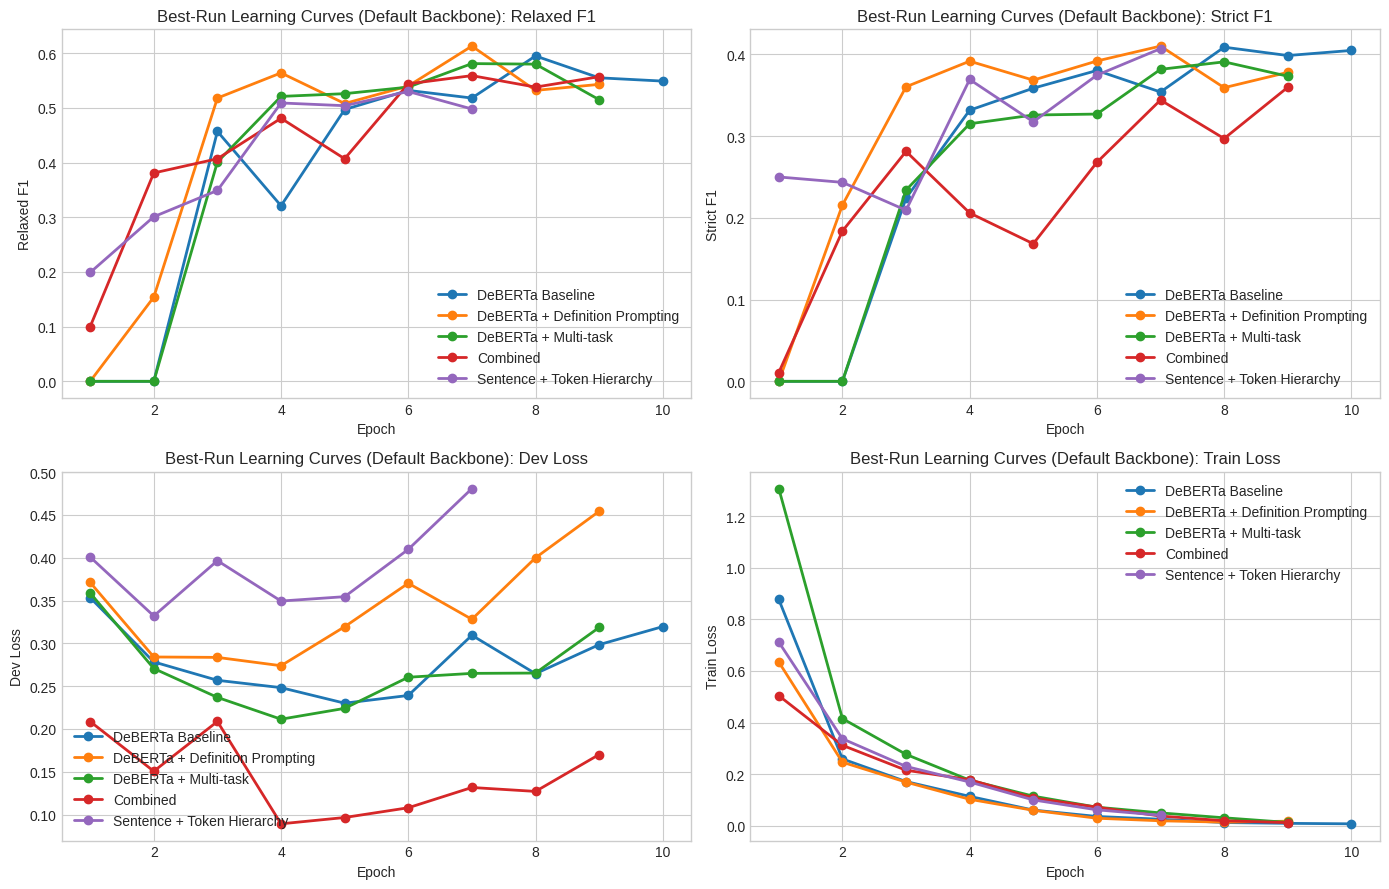
\includegraphics[width=\linewidth]{fig_training_curves.png}
\caption{Best-run learning curves. \textbf{Top row:} Definition prompting
(orange) tops both relaxed and strict F1 from epoch~4 onward, the
clearest single-recipe win. \textbf{Bottom row:} dev loss separates
recipes even when F1 curves look close; the Sentence~$+$~Token
Hierarchy drifts up after epoch~6, signaling mild overfit on this
small training set.}
\label{fig:curves}
\end{figure}

The learning-curve panel in Figure~\ref{fig:curves} makes the effect visible: definition prompting and the plain baseline plateau at $\approx 0.60$ relaxed F1, while other recipes oscillate around or below it. 
Dev loss is a noisier signal than F1 and sometimes separates recipes that F1 treats as similar (the Sentence~$+$~Token Hierarchy variant drifts up after epoch~6, which the raw F1 number does not show).

\subsection{Structured prediction pipelines}

Table~\ref{tab:pipelines} compares the four structured variants.
Hierarchical DeBERTa is the clear winner and becomes the anchor of our final ensemble. 
Strict F1 in the hierarchical pipeline actually goes up under preprocessing, even though relaxed F1 goes down: the sentence-gating head tightens predicted boundaries when the token head works with cleaner input.
The Two-Step Impact Pipeline trades recall for precision and posts a
strict F1 of $0.404$; its strict score sits below the preprocessed
DeBERTa baseline ($0.421$, Table~\ref{tab:core}) but above the
hierarchical pipeline, making it the strongest precision-oriented
structured variant in the sweep.

\begin{table}[t]
\centering\small
\begin{tabular}{l cc}
\toprule
Pipeline & Raw (R / S) & Prep (R / S) \\
\midrule
Hierarchical DeBERTa    & \textbf{0.604} / 0.372 & 0.559 / 0.383 \\
Two-Step Impact         & -- & 0.534 / 0.404 \\
Sentence $+$ Token      & -- & 0.530 / 0.375 \\
Span-nested GLiNER      & -- & 0.443 / 0.491 \\
\bottomrule
\end{tabular}
\caption{Structured prediction pipelines (dev F1). Only Hierarchical
DeBERTa was run under both regimes; the others are preprocessed only.}
\label{tab:pipelines}
\end{table}

\subsection{Model soup}

The best soup averages the top-$3$ checkpoints of the Recall-Boost
seed-42 LR sweep and reaches relaxed F1 $= 0.595$, i.e. exactly the
plain DeBERTa baseline, with strict F1 $0.331$ (the strict number is
worse). Soup recovers some of the damage from the Recall-Boost
experiment but does not exceed the unsouped baseline. This is
consistent with the findings of \citet{wortsman2022modelsoup}: soup
helps when the underlying recipe is already competitive, and does not rescue weaker recipes.

\subsection{Ensemble search}

Table~\ref{tab:ensemble} shows the top ensemble sizes from the cross-regime majority-vote search, plus the best probability-average result. The four-model majority ensemble achieves a relaxed F1 of $\textbf{0.635}$, a $+0.022$ jump over the best single model and $+0.025$ over the published baseline on the same dev split. The strict-F1 optimum is a different five-model subset at $0.518$. Hard voting consistently beats soft averaging on this benchmark ($0.635$ vs $0.614$), which is a reversal of the usual deep-learning preference for logit averaging.

\begin{table}[t]
\centering\scriptsize
\setlength{\tabcolsep}{4pt}
\begin{tabular}{lcccc}
\toprule
Ensemble & Relaxed & Strict & Prec. & Rec. \\
\midrule
2 models (majority)              & 0.623 & 0.465 & 0.586 & 0.664 \\
3 models (majority)              & 0.621 & 0.507 & 0.638 & 0.605 \\
\textbf{4 models (majority)}     & \textbf{0.635} & 0.509 & 0.648 & 0.623 \\
5 models (majority)              & 0.631 & \textbf{0.518} & 0.670 & 0.597 \\
\midrule
Prob.\ avg.\ (raw, 7 cand.)      & 0.614 & 0.431 & 0.653 & 0.580 \\
\bottomrule
\end{tabular}
\caption{Ensemble search. Cross-regime majority vote across $122{,}409$
size-2--5 subsets; probability average across $112$ size-2--5 subsets in the raw regime only (span/pipeline families are excluded because they
do not emit per-token distributions).}
\label{tab:ensemble}
\end{table}

The winning four-model subset pairs the Hierarchical DeBERTa pipeline
as an anchor with three complementary DeBERTa recipes drawn from both
preprocessing regimes: a definition-prompting run from the
preprocessed regime and two raw-regime runs with different
regularisation objectives. The ensemble benefits from both
\emph{preprocessing diversity} (members trained on different input
distributions) and \emph{objective diversity} (definition prompting,
multi-task, sentence gating), which is where the $+0.022$ headroom over the best single model comes from.

\subsection{Full ablation}

Table~\ref{tab:full} presents the full LR-selected ablation in one
view. BiLSTM--CRF sits at $0.296$; domain-adapted encoders underperform
the general-purpose DeBERTa; the only recipe that improves on the baseline alone is definition prompting; the four-model ensemble sits
clearly above the published SOTA on the same split.

\begin{table}[t]
\centering\small
\setlength{\tabcolsep}{5pt}
\begin{tabular}{lccc}
\toprule
Model & Relaxed & Strict & LR \\
\midrule
BiLSTM--CRF                               & 0.296 & 0.256 & 5e-4 \\
GLiNER (fine-tuned)                       & 0.524 & -- & 2e-5 \\
\ \ Span-nested GLiNER                    & 0.443 & -- & 1e-5 \\
SocBERT                                   & 0.404 & 0.277 & 5e-5 \\
StressRoBERTa                             & 0.482 & 0.270 & 2e-5 \\
DeBERTa baseline                          & 0.595 & 0.409 & 2e-5 \\
\ \ + Focal loss                          & 0.541 & 0.341 & 2e-5 \\
\ \ + Multi-task                          & 0.581 & 0.382 & 5e-5 \\
\ \ \textbf{+ Definition prompting}       & \textbf{0.613} & 0.410 & 5e-5 \\
Hierarchical DeBERTa                      & 0.604 & 0.372 & 2e-5 \\
Two-Step Impact                           & 0.534 & 0.404 & 2e-5 \\
Sentence + Token                          & 0.530 & 0.374 & 5e-5 \\
Recall-Boost (s42)                        & 0.582 & 0.312 & 2e-5 \\
R-Drop (s123)                             & 0.577 & 0.380 & 2e-5 \\
FGM + SWA (s42)                           & 0.573 & 0.356 & 2e-5 \\
Model soup (recall-boost s42)             & 0.595 & 0.331 & 2e-5 \\
\textbf{4-model majority ensemble}        & \textbf{0.635} & 0.509 & -- \\
\midrule
\textit{GPT-4o 3-shot (reported)}         & \textit{0.440} & -- & -- \\
\textit{DeBERTa published SOTA}           & \textit{0.610} & -- & -- \\
\bottomrule
\end{tabular}
\caption{Full LR-selected ablation (dev F1). Strict F1 for GLiNER
variants is not exposed by the toolkit. The GPT-4o 3-shot and
DeBERTa published SOTA numbers are the reference benchmarks reported by
the Reddit-Impacts 2.0 dataset release \citep{dey2025reddit}.}
\label{tab:full}
\end{table}

\section{Error Analysis}
\label{sec:error}

We ran a targeted error analysis on the best relaxed single model
(definition prompting, preprocessed regime, $\mathrm{lr}=5{\rm e}{-5}$,
relaxed F1 $= 0.613$, strict F1 $= 0.410$). Four categories dominate:

\paragraph{Boundary errors.} The $\approx 0.20$ gap between relaxed and strict F1 is almost entirely attributable to partial span matches on multi-word Social entities. Phrases such as ``charged with disorderly conduct'' are typed correctly, but the predicted span misses the ``charged with'' prefix.

\paragraph{Implicit false negatives.} Single-token implicit Clinical expressions (``hell'', ``broken'', ``numb'') and long-tail colloquial phrases are the dominant category of missed spans. These spans do not contain any clinical vocabulary, and the model falls back to the ``no-entity'' prior.

\paragraph{Negation handling.} Negated phrases are mostly rejected
correctly; type confusion between Clinical and Social is rare.

\paragraph{Third-person references.} The model over-rejects spans that
describe someone else's impacts rather than the poster's, despite no
explicit training signal for this distinction.

These categories suggest two concrete future-work directions:
boundary-aware decoding for the first category, and targeted synthetic
augmentation for the second.

\section{Discussion and Key Insights}
\label{sec:discussion}

Our headline finding is that \emph{training-objective diversity} is a
much stronger lever on this benchmark than individual-model polish. A
four-model majority-vote ensemble of relatively ordinary recipes beats
any single one of them by $+0.022$ relaxed F1. Three secondary
observations are worth calling out:

\paragraph{LR sweeps are non-negotiable.} The best LR is family-specific
($2{\rm e}{-5}$ for the plain baseline, $5{\rm e}{-5}$ for definition
prompting and multi-task). Running a single global LR would have
reversed the ordering between at least three recipes and hidden
definition prompting's improvement.

\paragraph{Domain adaptation is not a free lunch.} SocBERT and StressRoBERTa, both plausible a priori, underperform the best DeBERTa baseline (raw, $0.595$) by $0.113$ and $0.191$ relaxed F1 respectively---a $0.11$--$0.19$ gap. For a task whose labels are semantic categories defined at annotation time, generic language understanding appears to matter more than register-specific pre-training.

\paragraph{Majority vote beats probability average.} On our dev set hard voting is $+0.021$ better than soft averaging ($0.635$ vs $0.614$). We hypothesize that the most confident recipes are also the most over-confident: their logit mass dominates the average and propagates their particular mistakes, whereas a hard vote caps each member's influence at one. On a small, noisy benchmark with decorrelated errors, this cap is worth more than the information lost by discretizing the output.

\section{Limitations}
\label{sec:limit}

\paragraph{Dev-only evaluation.} We report dev-set performance
throughout. Test labels were not available during the study, and the
dev split itself is only $258$ documents, so a confidence interval on
relaxed F1 is wide. Given the $75\%\to 70\%$ label prior flip, test
numbers may well shift from what we report; the system rankings we
report are meaningful \emph{within} the dev distribution but do not
guarantee test-set generalization.

\paragraph{No cross-post context.} Our models see one post at a time.
User history within a subreddit is a potentially strong signal,
particularly for disambiguating third-person references, and we do not
exploit it.

\paragraph{Ensemble cost.} The best system runs four models at inference time and pays a $\approx 4\times$ latency penalty relative to a single-model deployment. In practice, the hierarchical pipeline at $0.604$ captures $\approx 0.03$ below the ensemble at a single-model cost.

\paragraph{Coverage of domain encoders.} Budget constraints restricted SocBERT and StressRoBERTa to the preprocessed regime only. It is possible---but in our view unlikely given the raw/prep ordering of the other transformers---that a raw run of either encoder would close the gap to DeBERTa.

\section{Conclusion}
\label{sec:conclusion}

We presented a systematic study of the Reddit-Impacts impact-extraction task, organized into seven contribution buckets layered atop a DeBERTa backbone, with a consistent LR sweep and a paired raw-vs-preprocessed protocol. Our best single model, definition prompting, achieves a relaxed F1 of 0.613. Our best system, a four-model majority-vote ensemble, reaches $0.635$ and exceeds the published baseline by $+0.025$ on the same dev split. The pattern across buckets is consistent: no single regularisation trick beats a well-tuned DeBERTa, and the headroom comes from combining decorrelated recipes via hard voting. We see the $\approx 0.18$ gap to the human ceiling as arising mainly from boundary decoding and implicit-expression recall, and view these as the most promising directions for future work.

\section*{Acknowledgments}

We thank the CE7455 course staff at NTU, and the SMM4H--HeaRD 2026
shared-task organizers for releasing Reddit-Impacts 2.0.

\bibliography{custom}

\appendix

\section{Hyperparameters and Training Setup}
\label{sec:hyperparams}

All DeBERTa-family runs use AdamW with $\beta = (0.9, 0.999)$,
weight decay $0.01$, batch size $16$, max sequence length $512$,
dropout $0.1$, linear warmup over $10\%$ of total steps, and linear
decay. LR is swept from $\{2{\rm e}{-5}, 5{\rm e}{-5}\}$. Training
runs for $12$ epochs unless otherwise noted; SWA averaging starts
after epoch $10$. BiLSTM--CRF trains with AdamW at learning rate
$5{\rm e}{-4}$ for up to $30$ epochs with early stopping (typically
converging around epoch~9). GLiNER fine-tuning follows the default schedule of
\citet{zaratiana2024gliner} with a $0.3$ span-score threshold.

\section{Reproducibility}
\label{sec:repro}

All experiments use PyTorch with mixed-precision training on a single
NVIDIA RTX A6000 GPU. The cross-regime ensemble search runs as a pure CPU
post-processing step on cached BIO sequences from each candidate and
takes roughly $45$ minutes for all $122{,}409$ size-2--5 subsets. The
probability-average search takes $\approx 5$ minutes on the 112
candidate subsets.

\end{document}
